\section{The Split Throughput Heuristic}
\label{sec:heuristic}

When initially considering which network scenarios to evaluate in our emulation
study, we discovered it to be non-trivial to pick scenarios that would lead to
a general understanding of the throughput of a congestion control scheme in a
split setting. It is challenging to select which network settings and
combinations of path segments to evaluate, as the parameter space for
combinations of path segments can be quite large. Also, not all CCA
implementations can be trivially split.

For this paper, we refer to \textit{throughput} as the throughput of a
long-lived data transfer in an emulated network, using a single flow.
We do not evaluate other metrics such as startup time, retransmission
overheads, or short-lived data transfers, which have been of interest to
PEPs and could also be impacted by connection-splitting.
When discussing throughput, we refer to \textit{end-to-end throughput} as
the throughput of an end-to-end connection, and \textit{split throughput} as the
throughput of the same connection when there is a connection-splitting PEP.

We realized that while split throughput is not necessarily well
understood for any combination of CCA, transport protocol, and network setting,
the end-to-end throughput often \textit{is}. We make the following insight
based on an ideal setting:

\begin{figure}[h]
  \centering
  \begin{tcolorbox}[colback=yellow!20, width=\linewidth, sharp corners]
    \textbf{Split Throughput Heuristic:} We can estimate the long-lived ``split
     throughput'' of a connection by measuring the long-lived ``end-to-end
     throughput'' on each segment of the split path and taking the minimum.
  \end{tcolorbox}
  \vspace{-0.3cm}
  \caption{\small A heuristic for evaluating split behavior from end-to-end behavior in
   an emulated network.}
  \label{fig:heuristic}
  \vspace{-0.1cm}
\end{figure}

\noindent Thus if we know the throughput of the much smaller parameter
 space of end-to-end connections, we can easily derive:

\begin{enumerate}[noitemsep]
    \item The split throughput of a CCA on a network path composed of two path
     segments,
    \item The end-to-end throughput on the network path,
    \item The expected throughput benefit of using a connection-splitting PEP
     on the network path.
\end{enumerate}

Furthermore, it is impossible to quantitatively evaluate the split throughput
of encrypted transport protocols without creating a custom and explicit
connection-splitting PEP. As a result, it is challenging to establish a
baseline for the throughput that is potentially achievable by QUIC with
in-network assistance, leaving many studies to compare QUIC only to split TCP~\cite
{thomas2019google,border2022evaluating,yuan2024sidekick}. The split throughput
heuristic allows us to estimate the throughput of encrypted transport
protocols using knowledge about its end-to-end throughput, without
actually splitting the connection.

In \Cref{sec:accuracy}, we discuss potential sources of error in the heuristic,
including the lack of consideration of the queue configuration on the proxy
or the placement of the bottleneck link relative to the data sender. However,
we believe there is a design tradeoff in accuracy versus simplicity.

In the rest of this section, we first describe how to use this heuristic to
analyze the split throughput benefit in a single network setting, without
having to run an emulation with a connection splitter. Then we describe how we
cache emulation results for an end-to-end parameter space to enable a more
open-ended analysis of CCAs over a variety of networks. Finally, we discuss the
limitations of our methodology using the heuristic, and propose possible
extensions.
% We use this heuristic to efficiently evaluate performance both with and without
% a PEP over an exhaustive parameter search of all practical combinations of two
% network path segments, within our model of a network in emulation.

% We use this understanding to develop a heuristic that extrapolates the benefits
% of connection-splitting based on the performance of the CCA in an end-to-end
% setting. Futhermore, we demonstrate how to quantify the extent of this benefit,
% which we call \textit{splittability}, in specific network settings and more
% broadly. We believe this heuristic model can help us better understand
% connection-splitting as an impactful technique for improving network
% performance, even as CCAs continue to evolve.


\subsection{Analyzing Split Throughput Benefit in a Single Network Setting}

\begin{lstfloat}[t]
\begin{lstlisting}[language=Python]
class NetworkModel:
    def __init__(self, delay, bw, loss):
        self.delay = delay
        self.bw = bw
        self.loss = loss

def compose(s1: NetworkModel,
            s2: NetworkModel) -> NetworkModel:
    delay = s1.delay + s2.delay
    bw = min(s1.bw, s2.bw)
    loss = s1.loss * (1-s1.loss)*s2.loss
    return NetworkModel(delay, bw, loss)

def throughput(s: NetworkModel) -> float:
    return run_emulation(s)
\end{lstlisting}
\vspace{-0.1cm}
\captionof{lstlisting}{\small An interface for modeling a network path and estimating
 throughput. The \texttt{compose()} function models an end-to-end network path
 from two path segments. The \texttt{throughput()} function obtains a throughput
 measurement for a path segment.}
\label{lst:multi-segment-network-model}
\vspace{-0.2cm}
\end{lstfloat}

\begin{lstfloat}[t]
\begin{lstlisting}[language=Python]
def pred_split_throughput(s1: NetworkModel,
                          s2: NetworkModel) -> float:
    return min(throughput(s1), throughput(s2))

def pred_e2e_throughput(s1: NetworkModel,
                        s2: NetworkModel) -> float:
    s = compose(s1, s2)
    return throughput(s)
\end{lstlisting}
\vspace{-0.1cm}
\captionof{lstlisting}{\small Functions that apply our simplified network model and the
 split throughput heuristic (\Cref{fig:heuristic}) to predict split and
 end-to-end throughput, using the interface in \Cref
 {lst:multi-segment-network-model}.}
\label{lst:pred-throughput-api}
\vspace{-0.2cm}
\end{lstfloat}

Given a network model of the two path segments that compose an end-to-end
network path, we would like to be able to estimate the expected throughput
benefit of using a connection-splitting PEP between the two segments. In our
emulation study, our simplified network model consists of three
parameters: delay, bandwidth, and loss.

We explicitly define the interface we
use to query split and end-to-end throughput in \Cref
{lst:multi-segment-network-model,lst:pred-throughput-api}. In addition
to the network model, we implement functions to \texttt{compose()} a model of
an end-to-end network path from two path segments and to
query the end-to-end \texttt{throughput()} of a segment.

\paragraph{The \texttt{compose()} function.}
Since our network model consists of three parameters, we describe how to compose
each of these parameters to model the end-to-end network path. Bandwidth is the
minimum of the two bandwidths, which is the bottleneck.
(We may also refer to ``bandwidth'' as ``link rate.'')
Delay is just additive.
If we think of loss as independent random loss, then the composition
of the two is $loss = loss1 + (1-loss1)\cdot loss2 = loss1 + loss2 -
loss1 \cdot loss2$.

Note that many combinations of path segments can compose to the same end-to-end
network path. This makes sense because regardless of where on the network path
loss occurs or which path segment has the bottleneck bandwidth, from an
end-to-end perspective, the network properties look the same.

\paragraph{The \texttt{throughput()} function.}
This is the throughput of a long-running HTTPS connection in a
\texttt{mininet} emulation. The emulated network is parameterized
by the network model of a single path segment, and the HTTPS implementation
uses the congestion control scheme of interest. We describe additional details
about the emulation in \Cref{sec:methodology}.
% emulation but with no hops instead of two, and a single
% emulator node to configure network properties. The client and server are the
% same, and the model of the network uses parameters in three dimensions: delay,
% link rate, and a random loss rate.

\paragraph{Calculating the split improvement.}

\Cref{lst:pred-throughput-api} demonstrates how we can estimate the split
throughput benefit using the interface in \Cref
{lst:multi-segment-network-model}. We \texttt{pred\_split\_throughput()} by taking
the minimum measured throughput on each network path segment, and \texttt
{pred\_e2e\_throughput()} by composing the path segments into an end-to-end
network path and using the measured throughput of that network path. The split
throughput benefit is just how much the split throughput has improved (if it has)
relative to the end-to-end throughput.

% \begin{figure}
    \centering
    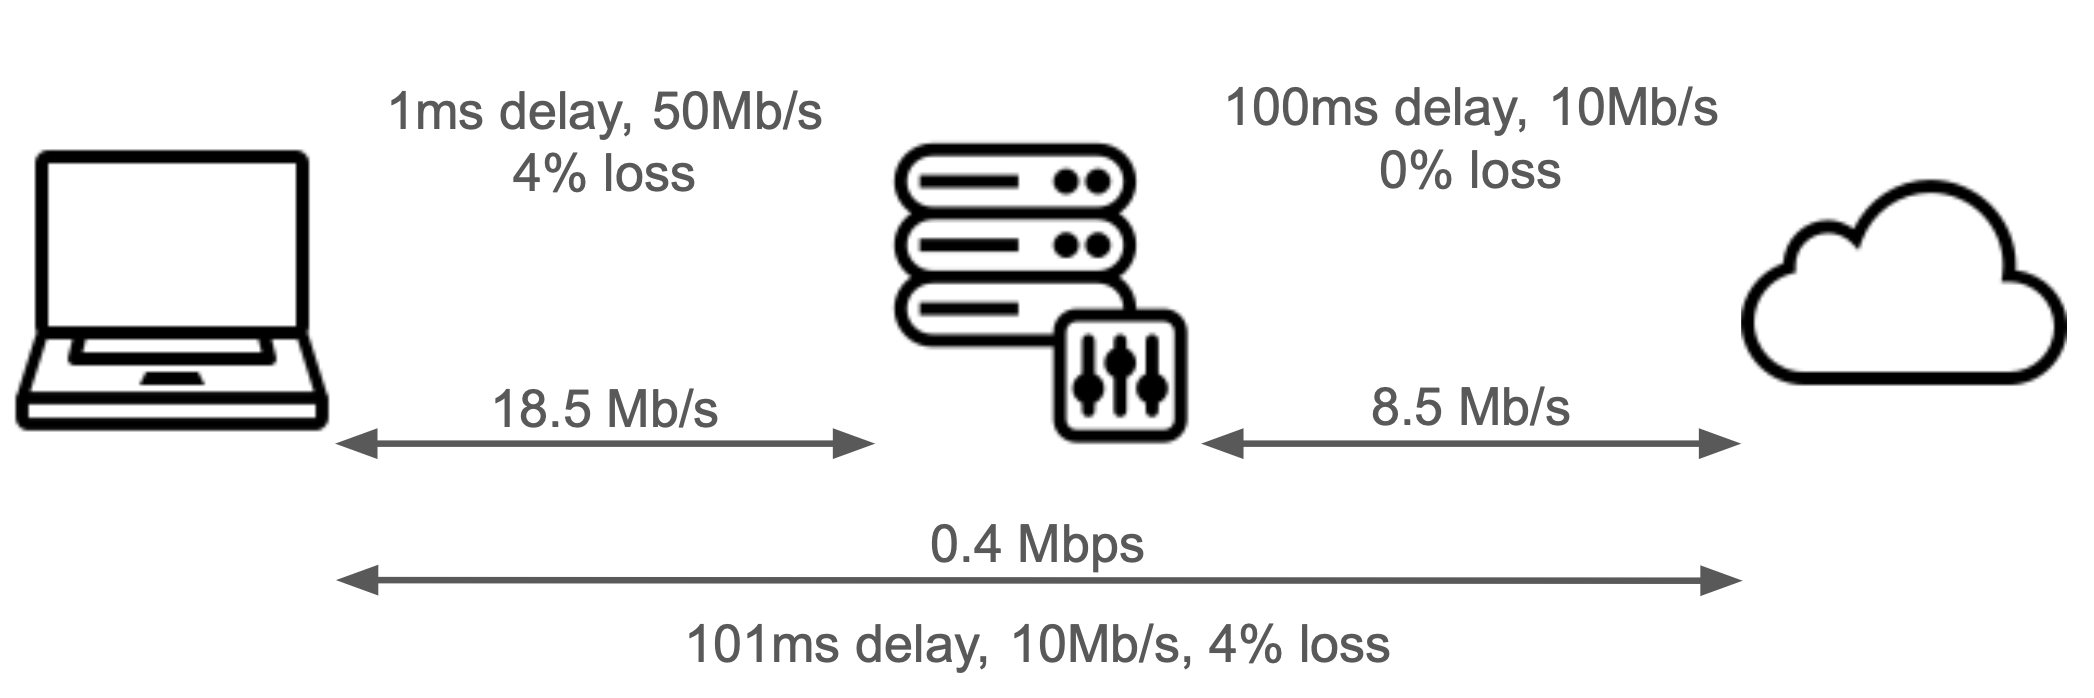
\includegraphics[width=\linewidth]{figures/heuristic_example.jpg}
    \caption{The predicted split throughput benefit is $\min(18.8, 8.5)/0.4 =
     21\times$. The goodput measurements are obtained by running end-to-end
     emulation experiments for each path segment and the composed network
     path.}
    \label{fig:heuristic-example}
\end{figure}


% \Cref{fig:heuristic-example} shows an explicit example of using the split
%  throughput heuristic to calculate the benefit of splitting in an
%  asymmetric network with a lossy last-mile.

\subsection{Caching Measurements for Analysis}
\label{sec:heuristic:caching}

While we can now predict split throughput for congestion control schemes which
are not easily
splittable, evaluating split throughput on a variety of network settings still
requires running emulations for each query. In order to speed up our analysis,
we select a parameter space of delay, bandwidth, and loss within our network
model and cache the end-to-end emulation results for this parameter space. We
describe our choice of parameter space and other modifications as follows:

\paragraph{Selecting a parameter space.} 
\begin{table}[t!]
  \centering
\begin{tabular}{ l l l l l }
  \toprule
    \textbf{Parameter} & \textbf{Values} & \textbf{Unit}\\
    \midrule
    Bandwidth & [10, 20, 30, 40, 50] & Mbit/s \\
    Delay & [1, 20, 40, 60, 80, 100] & ms \\
    Loss & [0, 1, 2, 3, 4] & \% \\
\bottomrule
\end{tabular}
  \caption{\small \label{tab:parameters} Network parameter space for the $5 \cdot
   6 \cdot 5 = 150$ combinations of network settings that we
   analyze in \Cref{sec:results}. These values attempt to realistically
   reflect network settings in which we'd see a PEP.}
   \vspace{-0.4cm}
\end{table}


We select a range of values we thought would realistically reflect network
settings in which we'd see a PEP (\Cref{tab:parameters}). We select propagation
delays from $1$ ms for a Wi-Fi last hop to $100$ ms to reflect the longer RTTs
of a satellite connection. Bottleneck bandwidths range from $10$ to $50$ Mbit/s
for a single connection, and are within the CPU constraints of emulation. Random
loss rates range from $0\%$ for a stable connection to $4\%$ for random loss
caused by e.g., wireless interference and extraterrestrial weather.

\paragraph{Modifying the \texttt{compose()} function.}
We make some subtle changes to the compose function to keep composed network
models within our parameter space.
In some sense, each parameter e.g., delay, can be thought of as an algebraic
group where the operator function is defined in \texttt{compose()}.

For path segments with small delays (1 ms),
we consider the composed path segment to
just have the delay of the longer segment, so we can have segments
with $1$ ms delay. For loss, note that when loss rates are small, $loss1 \cdot
loss2$ is negligibly small. In our case, the loss is always below $4\%$, so we
omit the term in the composition and loss becomes additive.

\paragraph{Collecting data efficiently.}
For some CCAs, we expect a large number of network settings in the parameter
space to have extremely low throughput. Thus we set a utilization threshold of
$5\%$ of the link rate below which we are not interested in the exact throughput
of that network setting.

To more efficiently build the cache, we run a search algorithm on
the parameter space to explore faster network settings first.
The initial network setting we evaluate has the lowest delay, bandwidth, and
loss. We explore adjacent data points if and only if the current data point has
not timed out.

% Since our experiments request a data size that takes $10$ seconds to transfer at
% maximum throughput, we set a worst case runtime of $180$ seconds for any
% experiment. For our parameter space above, there are a total of
% $5\cdot5\cdot5=125$ data points. The worst-case runtime for characterizing a
% CCA in our selected network space with a single trial per data point is
% $125\cdot180/60/60 \approx 6$ hours, and in practice much less.

\subsection{Limitations}
\label{sec:heuristic:limitations}

Although our methodology is more efficient for evaluating many network
settings and enables the exploration of theoretical scenarios,
caching measurements in emulation still takes non-negligible time. A much faster
method to estimate sustained throughput would be to use a theoretical model, such as the
TCP macroscopic model for AIMD schemes~\cite{mathis1997macroscopic}.
% , and to directly calculate the throughput from parameters in the network model.
However, this method does not reflect the nuances of implementation, and as
Mathis states himself, new models are needed for BBR and modern paradigms~\cite
{mathis2019deprecating,mathis2008reflections}.

Another limitation is our simplified network model and emulation testbed.
% However, we believe a more fundamental understanding of connection-splitting
% needs to start from somewhere, and propose extensions to the methodology.
One could incorporate more parameters into the network model, such as the
fluctuating bandwidths of cellular networks~\cite{hayes2019mmwave}, or how BBR
incorporates ACK aggregation~\cite{cardwell2018bbr-ietf101}. Another idea is to
generate end-to-end measurements from real testbeds instead of emulation. We
believe these challenges are not limited to emulation studies on split
performance, and hope to use the much more well-understood space of end-to-end
behavior to extrapolate split behavior.

% We acknowledge that we only test connections in a single-flow environment, and
% it is unclear how connection-splitting would impact fairness.
We acknowledge that we only test connections in a single-flow environment.
This limits what we can say about inter-flow fairness, but we can still infer
some aspects from how congestion-control schemes respond to loss and delay in
isolation, a classical concept known as ``TCP friendliness''~\cite{rfc5348}.
While split connections reduce retransmissions by buffering on the path,
their high throughput may also make them unfair. There may also be different
fairness implications when combining split with end-to-end connections.
% If eventually, connection-splitting becomes opt-in for
% some encrypted protocols or otherwise selective, it will be valuable to
% understand the fairness implications of combining split with end-to-end
% connections. On one hand, split connections reduce retransmission overheads by
% buffering on the path, but their high throughput may also make them unfair.
If every connection is split, then we refer to other studies for understanding
fairness at scale for each side of the concatenation~\cite
{philip2021revisiting}.

We also acknowledge that TCP is not limited to bulk data transfers, and that
it would be valuable to study other metrics that could be impacted by
connection-splitting, such as startup time, packet jitter, and retransmission
overheads.

Finally, our heuristic makes the simplified assumption that we can identify the
bottleneck path segment based on the minimum measured throughput. In reality,
the ability of a data sender to sustain that throughput depends on its ability
to saturate the send buffer. This is particularly true for data senders farther
along the network path, as their behavior will depend on the queue configuration
and the burstiness of previous senders. We explore this more in \Cref{sec:accuracy}.
% It would be interesting
% to explore how to incorporate these factors into the heuristic. It may be more
% challenging to model queue behavior in the real world as there are interactions
% with competing flows.
